% vim: set textwidth=78 autoindent:

% \subsection{GPS Plugin}\label{label_plugingps}
\subsection{Extension GPS}\label{label_plugingps}

% when the revision of a section has been finalized,
% comment out the following line:
% \updatedisclaimer

% \subsubsection{What is GPS?}\label{whatsgps}
\subsubsection{Qu'est ce qu'un GPS ?}\label{whatsgps}

% GPS, the Global Positioning System, is a satellite-based system that allows 
% anyone with a GPS receiver to find their exact position anywhere in the world.
% It is used as an aid in navigation, for example in airplanes, in boats and by 
% hikers.
Le GPS, Global Positioning System, est un système basé sur des satellites qui permet à toute personne possédant un récepteur GPS d'obtenir sa position exacte n'importe où dans le monde. Il est utilisé comme aide à la navigation, par exemple pour les avions, dans les bateaux et par les voyageurs.
% The GPS receiver uses the signals from the satellites to calculate its
% latitude, longitude and (sometimes) elevation.
Le récepteur GPS utilise les signaux des satellites pour calculer la latitude, la longitude et (parfois) l'élévation.
% Most receivers also have the capability to store locations (known as 
% \emph{waypoints}), sequences of locations that make up a planned \emph{route}
% and a tracklog or \emph{track} of the receivers movement over time.
La plupart des récepteurs ont également la possibilité de stocker la position (nommé \emph{waypoints}), des séquences de positions qui constituent un
\emph{itinéraire} prévu et un tracklog ou \emph{track} des déplacements du récepteur en fonction du temps.
% Waypoints, routes and tracks are the three basic feature types in GPS data.
% QGIS displays waypoints in point layers while routes and tracks are displayed
% in linestring layers.
Waypoints, itinéraires et tracks sont les trois types d'objet basic dans les données GPS. QGIs affiche les waypoints dans des couches points tandis que les itinéraires et les tracks sont affichés dans des couches linéaires.

% \subsubsection{Loading GPS data from a file}\label{label_loadgps}
\subsubsection{Charger des données GPS à partir d'un fichier}\label{label_loadgps}

% There are dozens of different file formats for storing GPS data.
Il y a des dizaines de formats de fichier différent pour stocker des données
GPS.
% The format that QGIS uses is called GPX (GPS eXchange format), which is a 
% standard interchange format that can contain any number of waypoints, routes
% and tracks in the same file.
Le format que QGIS utilise est appelé GPX (GPS eXchange format), qui est un format d'échange standard qui peut contenir n'importe quel nombre de waypoints, itinéraire et tracks dans un même fichier.

% To load a GPX file you first need to load the plugin \mainmenuopt{Plugins} >
% \dropmenuopttwo{mActionShowPluginManager}{Plugin Manager...} > \checkbox{GPS
% Tools}. When this plugin is loaded a button with a small handheld GPS device
% will show up in the toolbar. An example GPX file is available in the QGIS
% sample dataset: \filename{/qgis\_sample\_data/gps/national\_monuments.gpx}.
% See Section~\ref{label_sampledata} for more information about the sample data.
Pour charger un fichier GPX vous devez d'abord charger l'extension \mainmenuopt{Extensions} > \dropmenuopttwo{mActionShowPluginManager}{Gestionnaire
d'extensions} > \checkbox{Outils GPS}. Quand cette extension est chargée, un bouton avec un petit périphérique GPS apparaîtra dans la barre d'outils. Un fichier GPX d'exemple est disponible dans le jeu de données d'exemple de QGIS :
\filename{/qgis\_sample\_data/gps/national\_monuments.gpx}. Voir Section~\ref{label_sampledata} pour plus d'information sur les données d'exemple.

%\begin{enumerate}
%\item Click on the \toolbtntwo{gps_importer}{GPS Tools} icon and open the
%\tab{Load GPX file} tab (see figure \ref{figure gpxloader}).
%\item \button{Browse} to the folder \filename{qgis\_sample\_data/gps/},
%select the GPX file \filename{national\_monuments.gpx} and click \button{Open}.
%\end{enumerate}
\begin{enumerate}
\item cliquez sur l'icône \toolbtntwo{gps_importer}{Outils GPS} et ouvrez l'onglet \tab{Charger un fichier GPX} (voir figure \ref{figure gpxloader}).
\item \button{Naviguez} vers le répertoire \filename{qgis\_sample\_data/gps/}, sélectionnez le fichier GPX \filename{national\_monuments.gpx} et cliquez sur le bouton \button{Ouvrir}.
\end{enumerate}

\begin{figure}[ht]
   \begin{center}
% \caption{\label{gpxloader}The \emph{GPS Tools} dialog window \nixcaption}
\caption{\label{gpxloader}La boîte de dialogue de l'\emph{Outils GPS} \nixcaption}
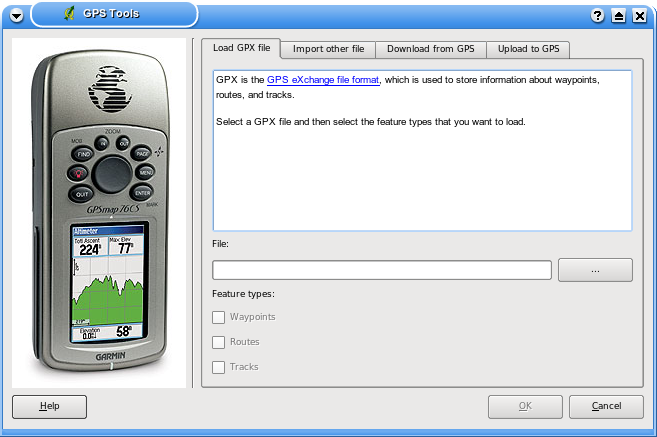
\includegraphics[clip=true, width=12cm]{loadgpx}
\end{center}
\end{figure}

% Use the browse button \browsebutton to select the GPX file, then use the
% checkboxes to select the feature types you want to load from that GPX file.
% Each feature type will be loaded in a separate layer when you click
% \button{OK}. The file \filename{national\_monuments.gpx} only includes
% waypoints.
Utilisez le bouton \browsebutton pour sélectionner le fichier GPX, puis utilisez la case à cocher pour sélectionner les types de géométrie que vous
voulez charger à partir de ce fichier GPX. Chaque type d'objet sera chargé dans une couche séparée lors du clique sur le bouton \button{OK}. Le fichier 
\filename{national\_monuments.gpx} inclue seulement des waypoints.

% \subsubsection{GPSBabel}
\subsubsection{GPSBabel}

% Since QGIS uses GPX files you need a way to convert other GPS file formats to
% GPX. This can be done for many formats using the free program GPSBabel, which
% is available at \url{http://www.gpsbabel.org}.
Puisque QGIs utilise des fichiers GPX vous avez besoin de convertir les autres formats de fichiers GPS en GPX. Cela peut être réalisé pour plusieurs formats en utilisant le logiciel libre GPSBabel qui est disponible sur \url{http://www.gpsbabel.org}.
% This program can also transfer GPS data between your computer and a GPS
% device. QGIS uses GPSBabel to do these things, so it is recommended that you
% install it. However, if you just want to load GPS data from GPX files you will
% not need it. Version 1.2.3 of GPSBabel is known to work with QGIS, but you
% should be able to use later versions without any problems.
Ce programme peut aussi transférer des données GPS entre votre ordinateur et un périphérique GPS. QGIS utilise GPSBabel pour réaliser ces tâches, il est donc recommandé de l'installer. Cependant si vous voulez juste charger des données à partir de fichiers GPX vous n'en avez pas besoin. La version 1.2.3 de GPSBabel est connue pour bien fonctionner avec QGIS, mais vous pouvez devriez pouvoir utiliser des versions plus récentes sans problème.

% \subsubsection{Importing GPS data}
\subsubsection{Importer des données GPS}

%To import GPS data from a file that is not a GPX file, you use the tool \tab{Import other file} in the GPS Tools dialog.
%Here you select the file that you want to import (and the file type), which feature type you want to import from it, where you want to store the converted GPX file and what the name of the new layer should be.  Note that not all GPS 
%data formats will support all three feature types, so for many formats 
%you will only be able to choose between one or two types. 
Pour importer des données d'un fichier qui n'est pas un fichier GPX, vous devez utiliser l'outil \tab{Importer d'autres fichiers} dans la boîte de dialogue des outils GPS. Vous sélectionnez le fichier que vous voulez importer, le type de géométrie vous voulez importer, l'emplacement où vous voulez stocker le fichier GPX converti et sous quel nom enregistrer la couche. Tous les formats de données GPS ne supportent pas les trois types d'entités, ne vous laissant le choix qu'entre un ou deux types.

% \subsubsection{Downloading GPS data from a device}
\subsubsection{Télécharger des données GPS à partir d'un périphérique}

%QGIS can use GPSBabel to download data from a GPS device directly as new vector layers.
%For this we use the \tab{Download from GPS} tab of the GPS Tools dialog (see Figure \ref{figure_download}). Here, we 
%select the type of GPS device, the port that it is connected to (or usb if your GPS supports this), the feature type that you want to download, the GPX file where the data should be stored, and the name of the new layer.

QGIS peut utiliser GPSBabel pour télécharger des données d'un périphérique GPS directement dans des couches vecteurs.
Pour cela, unous utilisons l'onglet \tab{Télécharger d'un GPS} de la fenêtre Outils GPS (voir figure~\ref{figure_download}). Vous y choisissez votre type de périphérique GPS, le port auquel il est connecté, le type de géométrie que vous voulez télécharger, le fichier GPX où les données doivent être stockées et le nom de la nouvelle couche.

\begin{figure}[ht]
   \begin{center}
% \caption{\label{figure_download}The download tool \nixcaption}
\caption{\label{figure_download}L'outil de téléchargement \nixcaption}
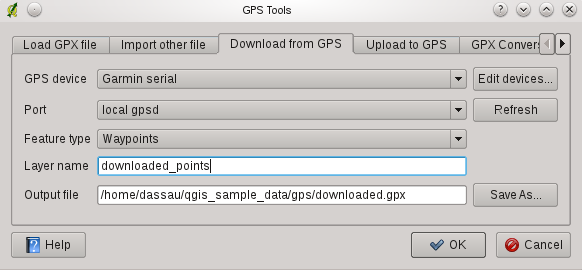
\includegraphics[clip=true, width=12cm]{download}
   \end{center}
\end{figure}

%The device type you select in the GPS device menu determines how GPSBabel tries to communicate with your GPS device.
%If none of the available types work with your GPS device you can create a new type (see section \ref{sec:Defining-new-device}).
Le type de périphérique que vous sélectionner dans le menu périphérique GPS détermine comme GPSBabel tente de communiquer avec votre périphérique GPS.
Si aucun des types ne fonctionne avec votre périphérique GPS, vous pouvez créer un nouveau type adapté (voir la section \ref{sec:Defining-new-device}).

%The port may be a file name or some other name that your operating system uses as a reference to the physical port in your computer that the GPS device is connected to. It may also be simply usb, for usb enabled GPS units.
Le port porte peut-être un nom de fichier ou un autre nom que votre système d'opération utiliserait comme une référence du port physique de votre ordinateur auquel le périphérique GPS est connecté. Il peut plus simplement être reconnu en USB dans le cas des appareils GPS équipés.
% \nix On Linux this is something like /dev/ttyS0 or /dev/ttyS1 and on \win 
% Windows it's COM1 or COM2.
\nix Sous Linux cela ressemble à /dev/ttyS0 ou /dev/ttyS1  et sous \win Windows c'est COM1 ou COM2.

% When you click \button{OK} the data will be downloaded from the device and 
% appear as a layer in QGIS.
Quand vous cliquez sur le bouton \button{OK} les données seront téléchargées du périphérique et apparaîtront dans une couche dans QGIS.

\subsubsection{Envoyer des données GPS vers un appareil}

%You can also upload data directly from a vector layer in QGIS to a GPS device using the \tab{Upload to GPS} tab of the GPS Tools dialog. To do this you simply select the layer that you want to upload (which must be a GPX layer), 
%your GPS device type, and the port (or usb) that it is connected to.
Vous pouvez également envoyer directement vos données depuis une couche vecteur de QGIS vers un périphérique GPS en utilisant l'oonglet \tab{Envoyer vers le GPS} de la fenêtre des Outils GPS (la couche doit être une couche GPX). Pour le faire, vous sélectionnez simplement la couche que vous voulez envoyer, le type de votre périphérique GPS et le port (com ou USB) auquel il est connecté.
% Just as with the download tool you can specify new device types if your device 
% isn't in the list.
De la même manière que pour l'outil de téléchargement, vous pouvez définir de nouveaux types de périphérique si le vôtre n'est pas dans la liste.

% This tool is very useful together with the vector editing capabilities of QGIS.
% You can load a map, create some waypoints and routes and then upload them and 
% use them in your GPS device.
%This tool is very useful in combination with the vector editing capabilities of QGIS. It allows you to load a map, create waypoints and routes, and then upload them and use them on your GPS device.
Cet outil est très utile lorsque combiné avec les capacités d'édition vectorielle de QGIS. Il permet de charger une carte, créer des points de passage, puis de les envoyer pour les utiliser dans votre périphérique GPS.

% \subsubsection{\label{sec:Defining-new-device}Defining new device types}
\subsubsection{\label{sec:Defining-new-device}Définir de nouveaux types de périphériques}

% There are lots of different types of GPS devices.
Il y a beaucoup de types différents de périphériques GPS.
% The QGIS developers can't test all of them, so if you have one that does not 
% work with any of the device types listed in the \tab{Download from GPS} and
% \tab{Upload to GPS} tools you can define your own device type for it.
Les développeurs de QGIS ne peuvent pas les tester tous, si vous en avez un qui ne fonctionne pas avec un des types de périphériques dans les outils
\tab{Récupérer du GPS} et \tab{Télécharger du GPS}, vous pouvez définir votre propre type de périphérique.
% You do this by using the GPS device editor, which you start by clicking the 
% \button{Edit devices} button in the download or the upload window.
Vous réalisez cela en utilisant l'éditeur de périphérique de GPS, que vous démarrez en cliquant le bouton \button{Éditer un périphérique} dans les
de téléchargement ou d'envoi.

% To define a new device you simply click the \button{New device} button, enter
% a name, a download command and an upload command for your device, and click
% the \button{Update device} button.
Pour définir un nouveau périphérique, vous cliquez sur le bouton \button{Nouveau périphérique}, entrez un nom, une commande de récupération et
une commande de téléchargement pour votre périphérique, et cliquez sur le bouton \button{Mise à jour du périphérique}.
% The name will be listed in the device menus in the upload and download
% windows, and can be any string.
Le nom sera listé dans les menus des périphériques dans la fenêtre récupération et téléchargement, et peut être n'importe quelle chaîne de caractère.
% The download command is the command that is used to download data from the 
% device to a GPX file.
La commande de récupération est la commande qui est utilisée pour récupérer les données du périphérique vers un fichier GPX.
% This will probably be a GPSBabel command, but you can use any other command 
% line program that can create a GPX file.
Ce sera certainement une commande GPSBabel, mais vous pouvez utiliser un autre programme en ligne de commande qui créé un fichier GPX.
% QGIS will replace the keywords \usertext{\%type}, \usertext{\%in}, and 
% \usertext{\%out} when it runs the command.
QGIS remplacera les mots-clé \usertext{\%type}, \usertext{\%in}, et \usertext{\%out} lorsqu'il lancera la commande.

% \usertext{\%type} will be replaced by {}``\usertext{-w}'' if you are 
% downloading waypoints, {}``\usertext{-r}'' if you are downloading routes and
% {}``\usertext{-t}'' if you are downloading tracks.
\usertext{\%type} sera remplacé par {}``\usertext{-w}''  si vous téléchargez des waypoints, {}``\usertext{-r}'' si vous téléchargez des routes et
{}``\usertext{-t}'' si vous téléchargez des tracks.
% These are command line options that tell GPSBabel which feature type to
% download.
Ce sont des options de la ligne de commande qui dit à GPSBabel quel type d'objet  à télécharger.

% \usertext{\%in} will be replaced by the port name that you choose in the 
% download window and \usertext{\%out} will be replaced by the name you choose 
% for the GPX file that the downloaded data should be stored in.
\usertext{\%in} sera remplacé par le port que vous avez choisi dans la boîte de dialogue de téléchargement et \usertext{\%out} sera remplacé par le nom que vous avez choisi pour le fichier GPX où les données téléchargées doivent être stockées.
% So if you create a device type with the download command
% {}``\usertext{gpsbabel\%type -i garmin -o gpx \%in \%out}'' (this is actually
% the download command for the predefined device type \selectstring{GPS
% device:}{Garmin serial})and then use it to download waypoints from port
% {}``\usertext{/dev/ttyS0}'' to the file {}``\usertext{output.gpx}'', QGIS will
% replace the keywords and run the command {}``\usertext{gpsbabel -w -i garmin
% -o gpx /dev/ttyS0 output.gpx}''.
Si vous créez un type de périphérique avec la commande de téléchargement {}``\usertext{gpsbabel\%type -i garmin -o gpx \%in \%out}'' (c'est actuellement
la commande de téléchargement pour le type de périphérique prédéfini \selectstring{GPS device:}{Garmin serial}) puis utilisez-le pour télécharger
les waypoints à partir du port {}``\usertext{/dev/ttyS0}''  vers le fichier {}``\usertext{output.gpx}'', QGIS remplacera les mots-clés et lancera la
commande {}``\usertext{gpsbabel -w -i garmin -o gpx /dev/ttyS0 output.gpx}''.

% The upload command is the command that is used to upload data to the device.
% The same keywords are used, but \usertext{\%in} is now replaced by the name of 
% the GPX file for the layer that is being uploaded, and \usertext{\%out} is
% replaced by the port name.
La commande de téléchargement est la commande qui est utilisée pour télécharger des données vers le périphérique. Le même mot-clé est utilisé, mais 
\usertext{\%in} est maintenant remplacé par le nom du fichier GPX pour la couche qui est en téléchargée et \usertext{\%out} est remplacé par le nom du port.

% You can learn more about GPSBabel and it's available command line options at 
% \url{http://www.gpsbabel.org}
Vous pouvez en savoir plus sur GPSBabel et ses options de ligne de commande disponible sur \url{http://www.gpsbabel.org}.

% Once you have created a new device type it will appear in the device lists
% for the download and upload tools.
Une fois le nouveau type de périphérique créé celui-ci apparaitra dans les listes de périphérique dans les outils de récupération et de téléchargement.

